\documentclass{beamer}

\usetheme{simple}

\usepackage{scalerel,xparse}
\usepackage{lmodern}
\usepackage[scale=2]{ccicons}
\usepackage{ulem}
\usepackage{tikz}
\usetikzlibrary{positioning,calc,automata}
\usepackage{algorithm}
\usepackage{algorithmic}
\usepackage{caption}
\usepackage{listings}
\usepackage{xcolor}

% Watermark background (simple theme)
\setlength{\parindent}{0cm}
\setwatermark{\includegraphics[height=8cm]{img/amogus.png}}


\title{\sout{CSC363} CSC369 Tutorial 6}
\subtitle{hope tomorrow's paul is feeling better!\\ (paul, having a headache and sick, on feb 23, while preparing slides)}
\date{\today}
\author{Paul ``sushi{\textunderscore}enjoyer'' Zhang}
\institute{University of Amogus}

\NewDocumentCommand\emojisushi{}{
    \includegraphics{img/1f363.png}
}
\NewDocumentCommand\emojiflushed{}{
    \includegraphics[scale=0.05]{img/1f633.png}
}  
\NewDocumentCommand\emojimoyai{}{
    \includegraphics{img/1f5ff.png}
}   

\begin{document}

\maketitle

\begin{frame}{Learning objectives this tutorial}
By the end of this tutorial, you should...
\begin{itemize}
\item Once again have CSIS (or whatever law enforcement for copyright violations in your jurisdiction) come to your house due to [REDACTED].
\item Have recalled the formal definition of a Turing machine, and have built one in Minecraft (or any other Turing-complete game)
\item Understand the formal definition of a multi-tape Turing machine, and have built one again in Minecraft (or any other Turing-complete game).
\item Understand the formal definition of a nondeterministic Turing machine.
\item Be infuriated by any further mentioning of computability, because we are completely done with that chapter of our lives.\footnote{If you hate computability, don't open assignment 3! (too bad you're forced to ;-;)}
\end{itemize}
\end{frame}

\begin{frame}{More unaffordable textbooks! yay :/}
\begin{figure}[h]
\centering
\includegraphics[width=9cm]{img/amazon.png}

i'm broke from spending money on sushi. i can't afford this textbook.
\end{figure}
Again, it's worth a read! you'll go over cool stuff like
\begin{itemize}
\item What really is a Turing machine? (3.1)
\item What are multi-tape and nondeterministic Turing machines? Why are they equivalent to Turing machines? (3.2)
\item What does $f(n) = O(g(n))$ mean again? What does $P$ mean? (7.1, 7.2)
\item Why didn't we use this textbook earlier? (69.420)
\end{itemize}
\end{frame}


\begin{frame}{Turing machines are back! :D}
Hope you remember what a Turing machine is! 

\begin{center}
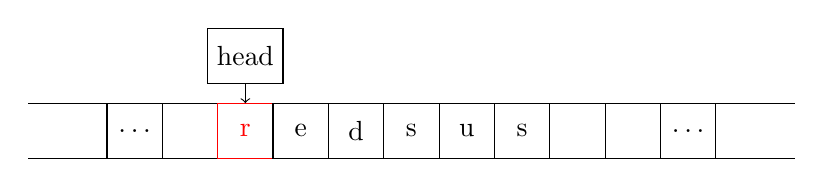
\begin{tikzpicture}[every node/.style={block},
        block/.style={minimum height=2em,minimum width=2em,outer sep=0pt,draw,rectangle,node distance=0pt}]
   \node (R1) {$\ldots$};
   \node (R2) [right=of R1] {$\square$};
   \node (R3) [right=of R2, color=red] {r};
   \node (R4) [right=of R3] {e};
   \node (R5) [right=of R4] {d};
   \node (R6) [right=of R5] {s};
   \node (R7) [right=of R6] {u};
   \node (R8) [right=of R7] {s};
   \node (R9) [right=of R8] {\emojiflushed};
   \node (R10) [right=of R9] {$\square$};
   \node (R11) [right=of R10] {$\ldots$};
   \node (HEAD) [above = 0.25cm of R3] {head};
   \draw[->] (HEAD) -- (R3);
   \draw (R1.north west) -- ++(-1cm,0) (R1.south west) -- ++ (-1cm,0);
   \draw (R11.north east) -- ++(1cm,0) (R11.south east) -- ++ (1cm,0);
\end{tikzpicture}
\end{center}
This Turing machine is sus \emojiflushed it only has one tape. what if we had multiple tapes?
\begin{center}
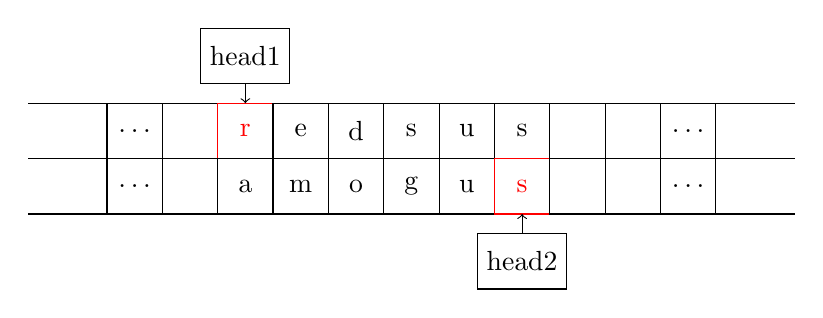
\begin{tikzpicture}[every node/.style={block},
        block/.style={minimum height=2em,minimum width=2em,outer sep=0pt,draw,rectangle,node distance=0pt}]
   \node (R1) {$\ldots$};
   \node (R2) [right=of R1] {$\square$};
   \node (R3) [right=of R2, color=red] {r};
   \node (R4) [right=of R3] {e};
   \node (R5) [right=of R4] {d};
   \node (R6) [right=of R5] {s};
   \node (R7) [right=of R6] {u};
   \node (R8) [right=of R7] {s};
   \node (R9) [right=of R8] {\emojiflushed};
   \node (R10) [right=of R9] {$\square$};
   \node (R11) [right=of R10] {$\ldots$};
   \draw (R1.north west) -- ++(-1cm,0) (R1.south west) -- ++ (-1cm,0);
   \draw (R11.north east) -- ++(1cm,0) (R11.south east) -- ++ (1cm,0);
   \node (R12) [below=of R1] {$\ldots$};
   \node (R13) [right=of R12] {$\square$};
   \node (R14) [right=of R13] {a};
   \node (R15) [right=of R14] {m};
   \node (R16) [right=of R15] {o};
   \node (R17) [right=of R16] {g};
   \node (R18) [right=of R17] {u};
   \node (R19) [right=of R18, color=red] {s};
   \node (R20) [right=of R19] {\emojiflushed};
   \node (R21) [right=of R20] {$\square$};
   \node (R22) [right=of R21] {$\ldots$};
   \draw (R12.north west) -- ++(-1cm,0) (R12.south west) -- ++ (-1cm,0);
   \draw (R22.north east) -- ++(1cm,0) (R22.south east) -- ++ (1cm,0);
   \node (HEAD1) [above = 0.25cm of R3] {head1};
   \draw[->] (HEAD1) -- (R3);
   \node (HEAD2) [below = 0.25cm of R19] {head2};
   \draw[->] (HEAD2) -- (R19);
\end{tikzpicture}
\end{center}

\end{frame}

\begin{frame}{Turing machines are back! :D}
\begin{center}
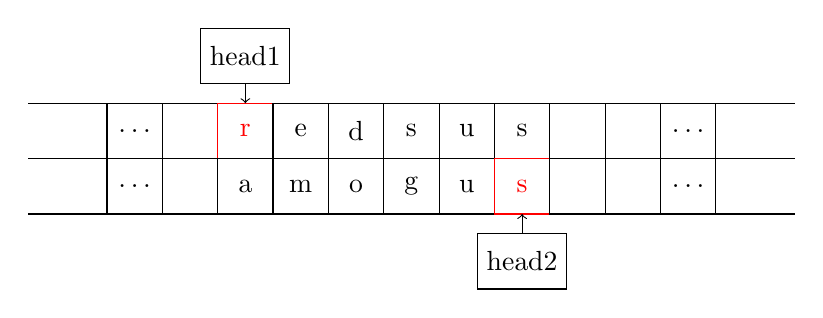
\begin{tikzpicture}[every node/.style={block},
        block/.style={minimum height=2em,minimum width=2em,outer sep=0pt,draw,rectangle,node distance=0pt}]
   \node (R1) {$\ldots$};
   \node (R2) [right=of R1] {$\square$};
   \node (R3) [right=of R2, color=red] {r};
   \node (R4) [right=of R3] {e};
   \node (R5) [right=of R4] {d};
   \node (R6) [right=of R5] {s};
   \node (R7) [right=of R6] {u};
   \node (R8) [right=of R7] {s};
   \node (R9) [right=of R8] {\emojiflushed};
   \node (R10) [right=of R9] {$\square$};
   \node (R11) [right=of R10] {$\ldots$};
   \draw (R1.north west) -- ++(-1cm,0) (R1.south west) -- ++ (-1cm,0);
   \draw (R11.north east) -- ++(1cm,0) (R11.south east) -- ++ (1cm,0);
   \node (R12) [below=of R1] {$\ldots$};
   \node (R13) [right=of R12] {$\square$};
   \node (R14) [right=of R13] {a};
   \node (R15) [right=of R14] {m};
   \node (R16) [right=of R15] {o};
   \node (R17) [right=of R16] {g};
   \node (R18) [right=of R17] {u};
   \node (R19) [right=of R18, color=red] {s};
   \node (R20) [right=of R19] {\emojiflushed};
   \node (R21) [right=of R20] {$\square$};
   \node (R22) [right=of R21] {$\ldots$};
   \draw (R12.north west) -- ++(-1cm,0) (R12.south west) -- ++ (-1cm,0);
   \draw (R22.north east) -- ++(1cm,0) (R22.south east) -- ++ (1cm,0);
   \node (HEAD1) [above = 0.25cm of R3] {head1};
   \draw[->] (HEAD1) -- (R3);
   \node (HEAD2) [below = 0.25cm of R19] {head2};
   \draw[->] (HEAD2) -- (R19);
\end{tikzpicture}
\end{center}
This 2-tape Turing machine will read in 2 symbols at once (as a 2-tuple), consult the current state, then output the following:
\begin{enumerate}
\item Next state to transition towards;
\item Symbol to write back via head1, and direction to move head1;
\item Symbol to write back via head2, and direction to move head2.
\end{enumerate}
\end{frame}



\begin{frame}{Greek letters are back! D:}
Do you like formal definitions? If you don't, too bad :(

\textbf{Task:} Recall that a Turing machine (the mathematical object) is an $8$-tuple $(Q, \Sigma, \Gamma, \delta, q_0, q_\text{accept}, q_\text{reject}, \square)$ where
\begin{itemize}
\item $Q$ is the (finite) set of states;
\item $\Sigma$ is the input alphabet not containing $\square$;
\item $\Gamma$ is the tape alphabet, and $\square \in \Gamma$ and $\Sigma \subseteq \Gamma$;
\item $\delta: Q \times \Gamma \to Q \times \Gamma \times \{L, R\}$ is the transition function;
\item $q_0 \in Q$ is the starting state;
\item $q_\text{accept}$ is the accept state;
\item $q_\text{reject}$ is the reject state (and $q_\text{reject} \neq q_\text{accept}$);
\item $\square$ is the blank symbol.
\end{itemize}
Familiarize yourself with this definition. Ask any questions you have!
\end{frame}

\begin{frame}{Greek letters are back! D:}
Do you like formal definitions? If you don't, too bad :(

\textbf{Task:} The definition of a $k$-tape Turing machine (the mathematical object) is an $8$-tuple $(Q, \Sigma, \Gamma, \delta, q_0, q_\text{accept}, q_\text{reject}, \square)$ where
\begin{itemize}
\item $Q$ is the (finite) set of states;
\item $\Sigma$ is the input alphabet not containing $\square$;
\item $\Gamma$ is the tape alphabet, and $\square \in \Gamma$ and $\Sigma \subseteq \Gamma$;
\item $\delta: Q \times \Gamma^k \to Q \times \Gamma^k \times \{L, R, -\}^k$ is the transition function;\footnote{$-$ is used to not move the head at all. This additional feature is not in the textbook definition of a $k$-tape Turing machine, but I added it as a user story in my spare time. Don't worry, the computational power is still equivalent.}
\item $q_0 \in Q$ is the starting state;
\item $q_\text{accept}$ is the accept state;
\item $q_\text{reject}$ is the reject state (and $q_\text{reject} \neq q_\text{accept}$);
\item $\square$ is the blank symbol.
\end{itemize}
Compare this with the previous definition. Ask any questions you have!
\end{frame}

\begin{frame}{Greek letters are back! D:}
But how does the $k$-tape Turing machine execute?

Here are the differences between a $k$-tape Turing machine and a regular Turing machine:
\begin{enumerate}
\item In a regular Turing machine, the string input is written on the (only) tape at the start of execution. In a $k$-tape Turing machine, the string input is always written on the first tape.
\item In a $k$-tape Turing machine, we read in $k$ symbols at once, and we output $k$ symbols and $k$ directions from $\{L, R, -\}$, to specify the symbol to write and direction to move for each of the $k$ tapes (where $-$ doesn't move it at all).
\item \texttt{helo\textunderscore fish.jpg} likes multi-tape Turing machines, unlike regular Turing machines.
\begin{figure}[h]
\centering
\includegraphics[width=5cm]{img/helo_fish.jpg}
\end{figure}
\end{enumerate}
\end{frame}

\begin{frame}{Let's try an example!}
I want to construct a 2-tape Turing machine will check if a given binary string is a palindrome. For example, $\emojisushi\emojimoyai\emojisushi\emojisushi\emojisushi\emojisushi\emojimoyai\emojisushi$ is accepted, while $\emojisushi\emojimoyai\emojimoyai\emojimoyai\emojisushi\emojimoyai\emojisushi\emojimoyai$ is not. 

\vspace{2mm}

Say we are given input $\emojisushi\emojisushi\emojimoyai\emojimoyai\emojimoyai\emojisushi\emojisushi$. The Turing machine would start out like so:

\begin{center}
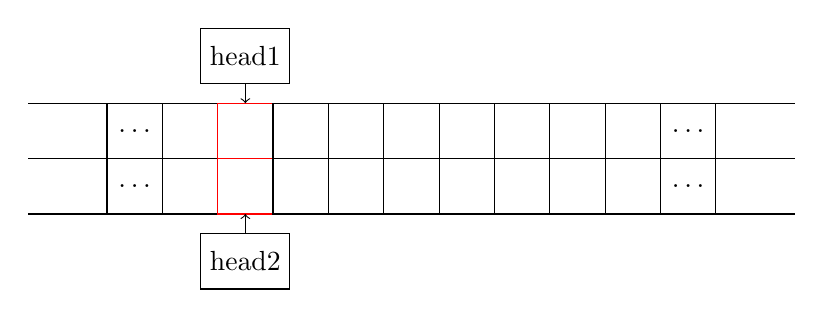
\begin{tikzpicture}[every node/.style={block},
        block/.style={minimum height=2em,minimum width=2em,outer sep=0pt,draw,rectangle,node distance=0pt}]
   \node (R1) {$\ldots$};
   \node (R2) [right=of R1] {$\square$};
   \node (R3) [right=of R2, color=red] {\emojisushi};
   \node (R4) [right=of R3] {\emojisushi};
   \node (R5) [right=of R4] {\emojimoyai};
   \node (R6) [right=of R5] {\emojimoyai};
   \node (R7) [right=of R6] {\emojimoyai};
   \node (R8) [right=of R7] {\emojisushi};
   \node (R9) [right=of R8] {\emojisushi};
   \node (R10) [right=of R9] {$\square$};
   \node (R11) [right=of R10] {$\ldots$};
   \draw (R1.north west) -- ++(-1cm,0) (R1.south west) -- ++ (-1cm,0);
   \draw (R11.north east) -- ++(1cm,0) (R11.south east) -- ++ (1cm,0);
   \node (R12) [below=of R1] {$\ldots$};
   \node (R13) [right=of R12] {$\square$};
   \node (R14) [right=of R13, color=red] {$\square$};
   \node (R15) [right=of R14] {$\square$};
   \node (R16) [right=of R15] {$\square$};
   \node (R17) [right=of R16] {$\square$};
   \node (R18) [right=of R17] {$\square$};
   \node (R19) [right=of R18] {$\square$};
   \node (R20) [right=of R19] {$\square$};
   \node (R21) [right=of R20] {$\square$};
   \node (R22) [right=of R21] {$\ldots$};
   \draw (R12.north west) -- ++(-1cm,0) (R12.south west) -- ++ (-1cm,0);
   \draw (R22.north east) -- ++(1cm,0) (R22.south east) -- ++ (1cm,0);
   \node (HEAD1) [above = 0.25cm of R3] {head1};
   \draw[->] (HEAD1) -- (R3);
   \node (HEAD2) [below = 0.25cm of R14] {head2};
   \draw[->] (HEAD2) -- (R14);
\end{tikzpicture}
\end{center}


\end{frame}

\begin{frame}{Let's try an example!}
\begin{center}
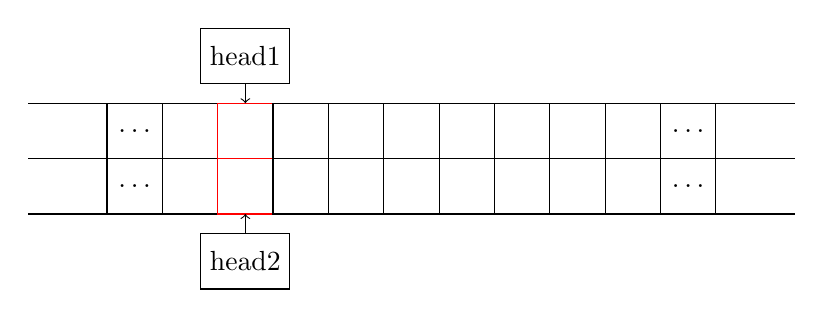
\begin{tikzpicture}[every node/.style={block},
        block/.style={minimum height=2em,minimum width=2em,outer sep=0pt,draw,rectangle,node distance=0pt}]
   \node (R1) {$\ldots$};
   \node (R2) [right=of R1] {$\square$};
   \node (R3) [right=of R2, color=red] {\emojisushi};
   \node (R4) [right=of R3] {\emojisushi};
   \node (R5) [right=of R4] {\emojimoyai};
   \node (R6) [right=of R5] {\emojimoyai};
   \node (R7) [right=of R6] {\emojimoyai};
   \node (R8) [right=of R7] {\emojisushi};
   \node (R9) [right=of R8] {\emojisushi};
   \node (R10) [right=of R9] {$\square$};
   \node (R11) [right=of R10] {$\ldots$};
   \draw (R1.north west) -- ++(-1cm,0) (R1.south west) -- ++ (-1cm,0);
   \draw (R11.north east) -- ++(1cm,0) (R11.south east) -- ++ (1cm,0);
   \node (R12) [below=of R1] {$\ldots$};
   \node (R13) [right=of R12] {$\square$};
   \node (R14) [right=of R13, color=red] {$\square$};
   \node (R15) [right=of R14] {$\square$};
   \node (R16) [right=of R15] {$\square$};
   \node (R17) [right=of R16] {$\square$};
   \node (R18) [right=of R17] {$\square$};
   \node (R19) [right=of R18] {$\square$};
   \node (R20) [right=of R19] {$\square$};
   \node (R21) [right=of R20] {$\square$};
   \node (R22) [right=of R21] {$\ldots$};
   \draw (R12.north west) -- ++(-1cm,0) (R12.south west) -- ++ (-1cm,0);
   \draw (R22.north east) -- ++(1cm,0) (R22.south east) -- ++ (1cm,0);
   \node (HEAD1) [above = 0.25cm of R3] {head1};
   \draw[->] (HEAD1) -- (R3);
   \node (HEAD2) [below = 0.25cm of R14] {head2};
   \draw[->] (HEAD2) -- (R14);
\end{tikzpicture}
\end{center}

We'll program the Turing machine to do the following, at a high level:
\begin{enumerate}
\item Copy the string on the first tape to the second tape.
\item Move head1 to the beginning of the first tape, and head2 to the last character on the second tape.
\item Compare the symbols at head1 and head2. If they are not equal, reject. Else move head1 to the right and head2 to the left. 
\end{enumerate}
\end{frame}

\begin{frame}
\begin{center}
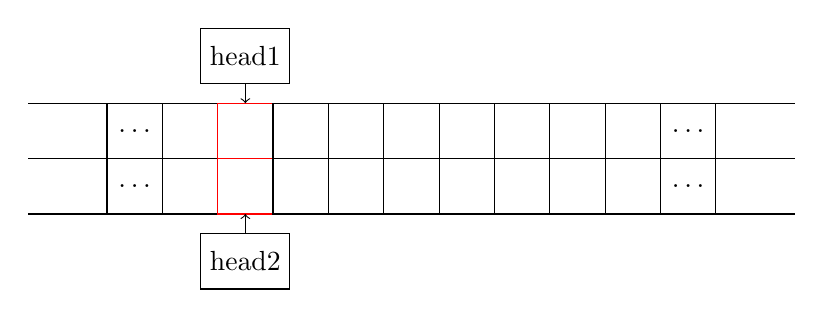
\begin{tikzpicture}[every node/.style={block},
        block/.style={minimum height=2em,minimum width=2em,outer sep=0pt,draw,rectangle,node distance=0pt}]
   \node (R1) {$\ldots$};
   \node (R2) [right=of R1] {$\square$};
   \node (R3) [right=of R2, color=red] {\emojisushi};
   \node (R4) [right=of R3] {\emojisushi};
   \node (R5) [right=of R4] {\emojimoyai};
   \node (R6) [right=of R5] {\emojimoyai};
   \node (R7) [right=of R6] {\emojimoyai};
   \node (R8) [right=of R7] {\emojisushi};
   \node (R9) [right=of R8] {\emojisushi};
   \node (R10) [right=of R9] {$\square$};
   \node (R11) [right=of R10] {$\ldots$};
   \draw (R1.north west) -- ++(-1cm,0) (R1.south west) -- ++ (-1cm,0);
   \draw (R11.north east) -- ++(1cm,0) (R11.south east) -- ++ (1cm,0);
   \node (R12) [below=of R1] {$\ldots$};
   \node (R13) [right=of R12] {$\square$};
   \node (R14) [right=of R13, color=red] {$\square$};
   \node (R15) [right=of R14] {$\square$};
   \node (R16) [right=of R15] {$\square$};
   \node (R17) [right=of R16] {$\square$};
   \node (R18) [right=of R17] {$\square$};
   \node (R19) [right=of R18] {$\square$};
   \node (R20) [right=of R19] {$\square$};
   \node (R21) [right=of R20] {$\square$};
   \node (R22) [right=of R21] {$\ldots$};
   \draw (R12.north west) -- ++(-1cm,0) (R12.south west) -- ++ (-1cm,0);
   \draw (R22.north east) -- ++(1cm,0) (R22.south east) -- ++ (1cm,0);
   \node (HEAD1) [above = 0.25cm of R3] {head1};
   \draw[->] (HEAD1) -- (R3);
   \node (HEAD2) [below = 0.25cm of R14] {head2};
   \draw[->] (HEAD2) -- (R14);
\end{tikzpicture}
\end{center}
1. Copy the string on the first tape to the second tape.
\begin{center}
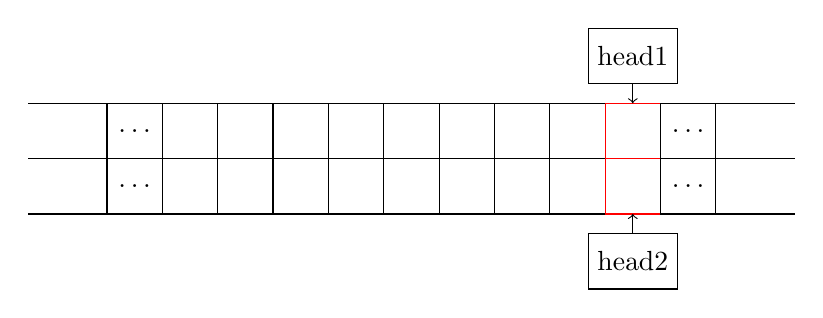
\begin{tikzpicture}[every node/.style={block},
        block/.style={minimum height=2em,minimum width=2em,outer sep=0pt,draw,rectangle,node distance=0pt}]
   \node (R1) {$\ldots$};
   \node (R2) [right=of R1] {$\square$};
   \node (R3) [right=of R2] {\emojisushi};
   \node (R4) [right=of R3] {\emojisushi};
   \node (R5) [right=of R4] {\emojimoyai};
   \node (R6) [right=of R5] {\emojimoyai};
   \node (R7) [right=of R6] {\emojimoyai};
   \node (R8) [right=of R7] {\emojisushi};
   \node (R9) [right=of R8] {\emojisushi};
   \node (R10) [right=of R9, color=red] {$\square$};
   \node (R11) [right=of R10] {$\ldots$};
   \draw (R1.north west) -- ++(-1cm,0) (R1.south west) -- ++ (-1cm,0);
   \draw (R11.north east) -- ++(1cm,0) (R11.south east) -- ++ (1cm,0);
   \node (R12) [below=of R1] {$\ldots$};
   \node (R13) [right=of R12] {$\square$};
   \node (R14) [right=of R13] {$\emojisushi$};
   \node (R15) [right=of R14] {$\emojisushi$};
   \node (R16) [right=of R15] {$\emojimoyai$};
   \node (R17) [right=of R16] {$\emojimoyai$};
   \node (R18) [right=of R17] {$\emojimoyai$};
   \node (R19) [right=of R18] {$\emojisushi$};
   \node (R20) [right=of R19] {$\emojisushi$};
   \node (R21) [right=of R20, color=red] {$\square$};
   \node (R22) [right=of R21] {$\ldots$};
   \draw (R12.north west) -- ++(-1cm,0) (R12.south west) -- ++ (-1cm,0);
   \draw (R22.north east) -- ++(1cm,0) (R22.south east) -- ++ (1cm,0);
   \node (HEAD1) [above = 0.25cm of R10] {head1};
   \draw[->] (HEAD1) -- (R10);
   \node (HEAD2) [below = 0.25cm of R21] {head2};
   \draw[->] (HEAD2) -- (R21);
\end{tikzpicture}
\end{center}
\end{frame}

\begin{frame}
\begin{center}
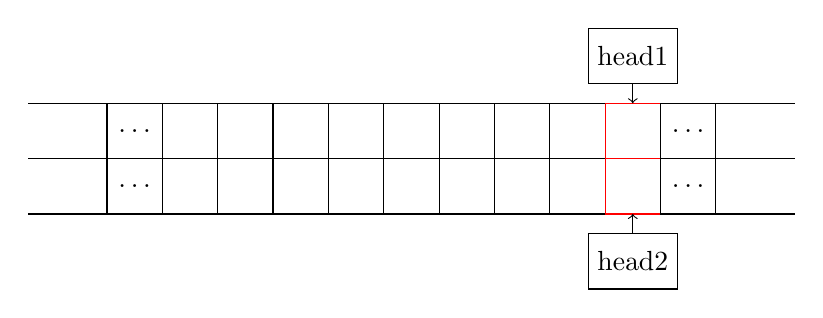
\begin{tikzpicture}[every node/.style={block},
        block/.style={minimum height=2em,minimum width=2em,outer sep=0pt,draw,rectangle,node distance=0pt}]
   \node (R1) {$\ldots$};
   \node (R2) [right=of R1] {$\square$};
   \node (R3) [right=of R2] {\emojisushi};
   \node (R4) [right=of R3] {\emojisushi};
   \node (R5) [right=of R4] {\emojimoyai};
   \node (R6) [right=of R5] {\emojimoyai};
   \node (R7) [right=of R6] {\emojimoyai};
   \node (R8) [right=of R7] {\emojisushi};
   \node (R9) [right=of R8] {\emojisushi};
   \node (R10) [right=of R9, color=red] {$\square$};
   \node (R11) [right=of R10] {$\ldots$};
   \draw (R1.north west) -- ++(-1cm,0) (R1.south west) -- ++ (-1cm,0);
   \draw (R11.north east) -- ++(1cm,0) (R11.south east) -- ++ (1cm,0);
   \node (R12) [below=of R1] {$\ldots$};
   \node (R13) [right=of R12] {$\square$};
   \node (R14) [right=of R13] {$\emojisushi$};
   \node (R15) [right=of R14] {$\emojisushi$};
   \node (R16) [right=of R15] {$\emojimoyai$};
   \node (R17) [right=of R16] {$\emojimoyai$};
   \node (R18) [right=of R17] {$\emojimoyai$};
   \node (R19) [right=of R18] {$\emojisushi$};
   \node (R20) [right=of R19] {$\emojisushi$};
   \node (R21) [right=of R20, color=red] {$\square$};
   \node (R22) [right=of R21] {$\ldots$};
   \draw (R12.north west) -- ++(-1cm,0) (R12.south west) -- ++ (-1cm,0);
   \draw (R22.north east) -- ++(1cm,0) (R22.south east) -- ++ (1cm,0);
   \node (HEAD1) [above = 0.25cm of R10] {head1};
   \draw[->] (HEAD1) -- (R10);
   \node (HEAD2) [below = 0.25cm of R21] {head2};
   \draw[->] (HEAD2) -- (R21);
\end{tikzpicture}
\end{center}
2. Move head1 to the beginning of the first tape, and head2 to the last character on the second tape.
\begin{center}
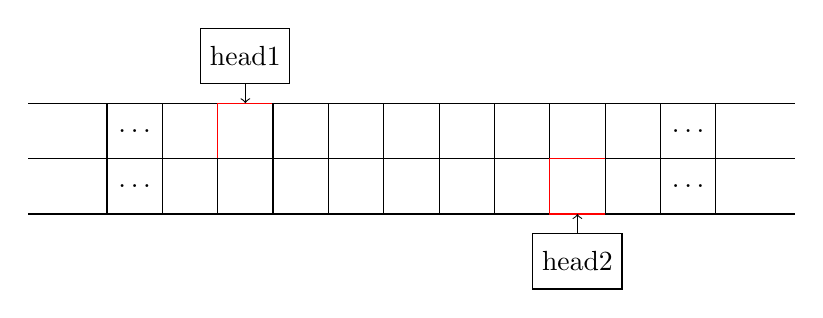
\begin{tikzpicture}[every node/.style={block},
        block/.style={minimum height=2em,minimum width=2em,outer sep=0pt,draw,rectangle,node distance=0pt}]
   \node (R1) {$\ldots$};
   \node (R2) [right=of R1] {$\square$};
   \node (R3) [right=of R2, color=red] {\emojisushi};
   \node (R4) [right=of R3] {\emojisushi};
   \node (R5) [right=of R4] {\emojimoyai};
   \node (R6) [right=of R5] {\emojimoyai};
   \node (R7) [right=of R6] {\emojimoyai};
   \node (R8) [right=of R7] {\emojisushi};
   \node (R9) [right=of R8] {\emojisushi};
   \node (R10) [right=of R9] {$\square$};
   \node (R11) [right=of R10] {$\ldots$};
   \draw (R1.north west) -- ++(-1cm,0) (R1.south west) -- ++ (-1cm,0);
   \draw (R11.north east) -- ++(1cm,0) (R11.south east) -- ++ (1cm,0);
   \node (R12) [below=of R1] {$\ldots$};
   \node (R13) [right=of R12] {$\square$};
   \node (R14) [right=of R13] {$\emojisushi$};
   \node (R15) [right=of R14] {$\emojisushi$};
   \node (R16) [right=of R15] {$\emojimoyai$};
   \node (R17) [right=of R16] {$\emojimoyai$};
   \node (R18) [right=of R17] {$\emojimoyai$};
   \node (R19) [right=of R18] {$\emojisushi$};
   \node (R20) [right=of R19, color=red] {$\emojisushi$};
   \node (R21) [right=of R20] {$\square$};
   \node (R22) [right=of R21] {$\ldots$};
   \draw (R12.north west) -- ++(-1cm,0) (R12.south west) -- ++ (-1cm,0);
   \draw (R22.north east) -- ++(1cm,0) (R22.south east) -- ++ (1cm,0);
   \node (HEAD1) [above = 0.25cm of R3] {head1};
   \draw[->] (HEAD1) -- (R3);
   \node (HEAD2) [below = 0.25cm of R20] {head2};
   \draw[->] (HEAD2) -- (R20);
\end{tikzpicture}
\end{center}
\end{frame}

\begin{frame}
\begin{center}
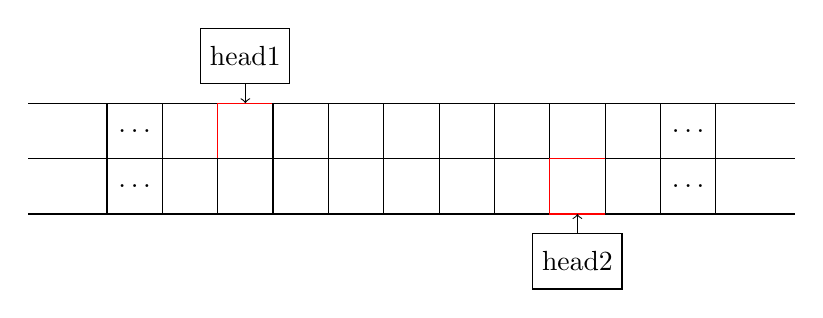
\begin{tikzpicture}[every node/.style={block},
        block/.style={minimum height=2em,minimum width=2em,outer sep=0pt,draw,rectangle,node distance=0pt}]
   \node (R1) {$\ldots$};
   \node (R2) [right=of R1] {$\square$};
   \node (R3) [right=of R2, color=red] {\emojisushi};
   \node (R4) [right=of R3] {\emojisushi};
   \node (R5) [right=of R4] {\emojimoyai};
   \node (R6) [right=of R5] {\emojimoyai};
   \node (R7) [right=of R6] {\emojimoyai};
   \node (R8) [right=of R7] {\emojisushi};
   \node (R9) [right=of R8] {\emojisushi};
   \node (R10) [right=of R9] {$\square$};
   \node (R11) [right=of R10] {$\ldots$};
   \draw (R1.north west) -- ++(-1cm,0) (R1.south west) -- ++ (-1cm,0);
   \draw (R11.north east) -- ++(1cm,0) (R11.south east) -- ++ (1cm,0);
   \node (R12) [below=of R1] {$\ldots$};
   \node (R13) [right=of R12] {$\square$};
   \node (R14) [right=of R13] {$\emojisushi$};
   \node (R15) [right=of R14] {$\emojisushi$};
   \node (R16) [right=of R15] {$\emojimoyai$};
   \node (R17) [right=of R16] {$\emojimoyai$};
   \node (R18) [right=of R17] {$\emojimoyai$};
   \node (R19) [right=of R18] {$\emojisushi$};
   \node (R20) [right=of R19, color=red] {$\emojisushi$};
   \node (R21) [right=of R20] {$\square$};
   \node (R22) [right=of R21] {$\ldots$};
   \draw (R12.north west) -- ++(-1cm,0) (R12.south west) -- ++ (-1cm,0);
   \draw (R22.north east) -- ++(1cm,0) (R22.south east) -- ++ (1cm,0);
   \node (HEAD1) [above = 0.25cm of R3] {head1};
   \draw[->] (HEAD1) -- (R3);
   \node (HEAD2) [below = 0.25cm of R20] {head2};
   \draw[->] (HEAD2) -- (R20);
\end{tikzpicture}
\end{center}
Compare the symbols at head1 and head2. If they are not equal, reject. Else move head1 to the right and head2 to the left. 
\end{frame}

\begin{frame}
I want to construct a 2-tape Turing machine will check if a given binary string is a palindrome. For example, $\emojisushi\emojimoyai\emojisushi\emojisushi\emojisushi\emojisushi\emojimoyai\emojisushi$ is accepted, while $\emojisushi\emojimoyai\emojimoyai\emojimoyai\emojisushi\emojimoyai\emojisushi\emojimoyai$ is not. 

\vspace{2mm}

We'll program the Turing machine to do the following, at a high level:
\begin{enumerate}
\item Copy the string on the first tape to the second tape.
\item Move head1 to the beginning of the first tape, and head2 to the last character on the second tape.
\item Compare the symbols at head1 and head2. If they are not equal, reject. Else move head1 to the right and head2 to the left. 
\end{enumerate}

\textbf{Task:} \sout{Formally write out this Turing machine.}

Go to \url{https://turingmachinesimulator.com}, load the ``Fast binary palindrome'' example under ``Examples''.\footnote{Or just click here: \url{http://turingmachinesimulator.com/shared/pxgabhhejv}} Try to understand what is going on here! Ask questions!
\end{frame}

\begin{frame}{Why is this relevant?}
\sout{Cuz I was told to cover this in tutorial} Because they are actually equivalent in computational power! (not exactly, but they are kinda equivalent)

\vspace{2mm}

By that we mean something is ``computable'' by a regular Turing machine if and only if it is ``computable'' by a multi-tape Turing machine, whatever reasonable definition of ``computable'' you use.

\begin{figure}[h]
\centering
\includegraphics[width=8cm]{img/morshu.jpg}

(not actually gonna do it, it's in the textbook though!)
\end{figure}
\end{frame}

\begin{frame}{Why is this relevant?}

\vspace{2mm}

They aren't necessarily equivalent in terms of \textit{computational complexity} though.\footnote{By computational complexity, I mean the \textit{number of steps} it takes to halt. Refer to CSC236/CSC263 or whatever, lol.}\\

\vspace{2mm}

Our $2$-tape Turing machine takes $O(n)$ steps to determine whether a string of length $n$ is a palindrome or not. In a regular Turing machine, we're probably gonna need $O(n^2)$ steps. So in some sense, multi-tape Turing machines are more efficient at computation!

\vspace{2mm}

\begin{figure}[h]
\centering
\includegraphics[width=5cm]{img/average.jpg}
\end{figure}


\end{frame}

\begin{frame}{Why is this relevant?}

there's a nice theorem in the textbook! (chapter 7, theorem 7.8)

\begin{theorem}[kinda]
If something is computable in $t(n)$ time by a multi-tape Turing machine, then it is also computable in $O((t(n))^2)$ time by a regular Turing machine.
\end{theorem}

you don't need to fully understand what this means! informally it's just saying whatever a multi-tape Turing machine can do, a regular Turing machine can do as well, but possibly slower!

\begin{figure}[h]
\centering
\includegraphics[width=5cm]{img/average2.jpg}
\end{figure}

\end{frame}

\begin{frame}{break!}

pls dont copyright strike me, kero kero bonito sama uwu

\url{https://www.youtube.com/watch?v=PEmqJBcQ2lg}

\begin{figure}[h]
\centering
\includegraphics[width=12cm]{img/ao.png}
\end{figure}
\end{frame}

\begin{frame}{non-deterministic turing machines!}
because sometimes, just like humans, turing machines can't make up their minds ;-;

\vspace{2mm}

Remember DFAs and NFAs from CSC236? Me neither. But there's a good analogy between $$\text{Turing Machine : Nondeterministic Turing Machine}$$
and
$$\text{DFA : NFA}$$
In a Nondeterministic Turing machine, there are multiple possible execution paths!
\end{frame}

\begin{frame}{Greek letters are back, once again!}
Do you like formal definitions? If you don't, too bad :(

\textbf{Task:} The definition of a nondeterministic Turing machine (the mathematical object) is an $8$-tuple $(Q, \Sigma, \Gamma, \delta, q_0, q_\text{accept}, q_\text{reject}, \square)$ where
\begin{itemize}
\item $Q$ is the (finite) set of states;
\item $\Sigma$ is the input alphabet not containing $\square$;
\item $\Gamma$ is the tape alphabet, and $\square \in \Gamma$ and $\Sigma \subseteq \Gamma$;
\item {\color{red}$\delta \subseteq (Q \times \Gamma) \times (Q \times \Gamma \times \{L, R\})$ is the transition \textbf{relation};}
\item $q_0 \in Q$ is the starting state;
\item $q_\text{accept}$ is the accept state;
\item $q_\text{reject}$ is the reject state (and $q_\text{reject} \neq q_\text{accept}$);
\item $\square$ is the blank symbol.
\end{itemize}
Take a moment to understand why $\delta \subseteq (Q \times \Gamma) \times (Q \times \Gamma \times \{L, R\})$ instead of $\delta: Q \times \Gamma \to Q \times \Gamma \times \{L, R\}$. Ask questions!
\end{frame}

\begin{frame}{How does a nondeterministic Turing machine accept some input?}

A nondeterministic Turing machine $M$ \textbf{accepts} input $x$ when $M$ has \textit{some} execution path that halts in an accepting state. 

\vspace{2mm}

An analogy: We say an awkward CS student $p$ is \textbf{successful} in their job application when there is \textit{some} company $C$ that $p$ has applied to, for which $C$ has offered $p$ an internship.\footnote{Even if $C$ is underpaying $p$, which happens all the time, unfortunately :(}
\end{frame}

\begin{frame}{The \textit{POWER} of nondeterministic Turing machines (at a high level)}
unfortunately i won't be going over any low-level examples of nondeterministic Turing machines today :(

\vspace{2mm}

\textbf{Subset Sum Problem:} Given a set of integers $S = \{s_1, s_2, \ldots, s_n\}$ and a \textit{target sum} $T$, write a program (a Turing machine) to determine if $S$ has a subset $S' \subseteq S$ such that the sum of $S'$, $\sum S'$, is equal to $T$. 

\vspace{2mm}

For example, say we are given $S = \{1, 2, 3, 4, 5, 6\}$, and $T = 11$. Then the program should say ``yes'', because there exists a subset $S' \subseteq S$ such that $\sum S' = T$: if we take $S' = \{1, 2, 3, 5\}$ then $\sum S' = 11$.

\vspace{2mm}

For example, say we are given $S = \{5, 5, 5, 6, 6, 6\}$, and $T = 13$. Then the program should say ``no'', because there does not exist a subset $S' \subseteq S$ such that $\sum S' = T$. You can convince yourself by \textit{checking every subset of $S$}.

\vspace{2mm}

\textbf{Task:} Write a program (a Turing machine) that solves the Subset Sum Problem (i.e. given $S$ and $T$, return \texttt{true} iff $S$ has a subset $S'$ such that $\sum S' = T$). Use Pseudocode!

\end{frame}

\begin{frame}{The \textit{POWER} of nondeterministic Turing machines (at a high level)}
\textbf{Answer:} something like
\begin{align*}
& \text{Subset-Sum($S$, $T$):}\\
& \quad \text{For all $2^n$ subsets $S' \subseteq S$:}\\
& \quad \quad \text{if $\sum S' = T$: }\\
& \quad \quad \quad \text{return \texttt{true}}\\
& \quad \text{return \texttt{false}}\\
\end{align*}

This code is very inefficient: it has to go through all $2^n$ subsets of $S$! Can we do any better? 

\textbf{Task:} Answer the above.

\end{frame}

\begin{frame}{The \textit{POWER} of nondeterministic Turing machines (at a high level)}
lol if you've managed to successfully answer the above, you get one million dollars!\footnote{and possibly have just become the world's greatest computer scientist/mathematician, and also break all feasible encryption systems used today, allowing you to hack into bank accounts, and become a modern trillionaire, and the greatest villain of all time. so you no longer have to illegally [REDACTED] textbooks, and have an infinite supply of sushi \emojisushi \emojisushi \emojisushi (or whatever your fav food is).} answering that question amounts to solving $P = NP$ (but you don't need to know what that means for now).
 
\end{frame}

\begin{frame}{The \textit{POWER} of nondeterministic Turing machines (at a high level)}
We can do better with nondeterministic Turing machines! \footnote{unfortunately this isn't really practical in real life, so no infinite sushi supply yet :(}

Define the nondeterministic Turing machine $M$ using the following pseudocode:
\begin{align*}
& \text{Subset-Sum($S$, $T$):}\\
& \quad \textbf{Choose a particular subset $S' \subseteq S$:}\\
& \quad \text{if $\sum S' = T$: }\\
& \quad \quad \text{return \texttt{true}}\\
& \quad\text{return \texttt{false}}
\end{align*}
\textbf{Task:} Answer the following:
\begin{enumerate}
\item \small{}Why is the above code is allowed (as a high-level description of a nondeterministic Turing machine)?
\item Why is it that $M$ accepts $(S, T)$ if and only if $(S, T)$ satisfies the subset sum problem? Recall what it means for a nondeterministic $M$ to accept an input.
\end{enumerate}

\end{frame}

\begin{frame}{end i think?}
hey, uh, sorry if today's tutorial seemed pretty rushed! you don't have to fully understand what a multi-tape turing machine or a nondeterministic turing machine is, as long as you get the high level concepts:
\begin{itemize}
\item multi-tape turing machines read and write multiple symbols at once
\item whatever a multi-tape turing machine can compute, a regular turing machine can compute as well (possibly taking more time to compute)
\item nondeterministic turing machines can have multiple different execution paths (think of it like alternate universes!), and are more efficient than regular turing machines, but aren't really practical in real life unfortunately :/
\item big chungus is gone, i am sick, and i don't know what i'm writing for these slides anymore
\end{itemize}
\end{frame}

\end{document}